\ifnum \Version=1
\question[7] Use the method of reduction of order to find a second solution $y_2$ of the given differential equation such that $\{y_1, y_2\}$ is a fundamental set of solutions on the given interval. $$t^2y'' - t(t+2)y' + (t+2)y=0, \quad t > 0 , \quad y_1(t) = t$$
\ifnum \Solutions=1 {\color{DarkBlue} Solution written below. 
    \begin{figure}[h]
    \centering
    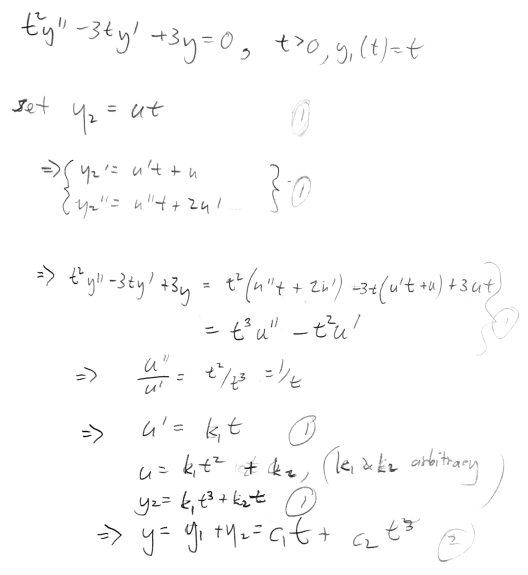
\includegraphics[width=14cm]{Images/ImgTest2RoO.png}
    \end{figure}  
} 
\else 
\vspace{3cm}
\fi
\fi 

\ifnum \Version=2
\question[7] Determine the general solution to the differential equation. 
$$y'' +4y'+3y = 18t+33, \quad y=y(t)$$
\ifnum \Solutions=1 {\color{DarkBlue} \\[12pt] 
The homogeneous equation has the characteristic equation
$$\lambda ^2+4\lambda + 3 = 0$$
The roots are $\lambda= -1$, $\lambda = -3$, so the homogeneous solution is
$$y_h = c_1 e^{-t} + c_2 e^{-3t} $$
We can use undetermined coefficients to identify the particular solution. With undetermined coefficients we can try a solution of the form $y_p = At+B$. To substitute this expression for the particular solution to the given differential equation, we differentiate twice to obtain:
\begin{align}
    y_p ' &=  A \\
    y_p'' &= 0
\end{align}
Substituting these expressions into the differential equation we have:
\begin{align}
    0 &= y'' + 4y' + 3y \\
    0 &= 0 + 4A +3(At+B)
\end{align}
By comparison, we obtain
$$ 3A = 18, 4A+3B = 33$$
Thus $A=6$ and $B=3$
The full solution to the DE is
$$y = y_h + y_p = c_1y_1  + c_2y_2 + y_p = c_1e^{-t} + c_2 e^{-3t} + 6t+3$$
} 
\else 
\vspace{3cm}
\fi
\fi 

\ifnum \Version=3
\question[7] Determine the general solution to the differential equation. 
$$y'' +4y'+3y = 18t+33, \quad y=y(t)$$
\ifnum \Solutions=1 {\color{DarkBlue} \\[12pt] 
The homogeneous equation has the characteristic equation
$$\lambda ^2+4\lambda + 3 = 0$$
The roots are $\lambda= -1$, $\lambda = -3$, so the homogeneous solution is
$$y_h = c_1 e^{-t} + c_2 e^{-3t} $$
We can use undetermined coefficients to identify the particular solution. With undetermined coefficients we can try a solution of the form $y_p = At+B$. To substitute this expression for the particular solution to the given differential equation, we differentiate twice to obtain:
\begin{align}
    y_p ' &=  A \\
    y_p'' &= 0
\end{align}
Substituting these expressions into the differential equation we have:
\begin{align}
    0 &= y'' + 4y' + 3y \\
    0 &= 0 + 4A +3(At+B)
\end{align}
By comparison, we obtain
$$ 3A = 18, 4A+3B = 33$$
Thus $A=6$ and $B=3$
The full solution to the DE is
$$y = y_h + y_p = c_1y_1  + c_2y_2 + y_p = c_1e^{-t} + c_2 e^{-3t} + 6t+3$$
} 
\else 
\vspace{3cm}
\fi
\fi 


\ifnum \Version=4
\question[7] Determine the general solution to the differential equation. 
$$y'' +4y'+3y = 18t+33, \quad y=y(t)$$
\ifnum \Solutions=1 {\color{DarkBlue} \\[12pt] 
The homogeneous equation has the characteristic equation
$$\lambda ^2+4\lambda + 3 = 0$$
The roots are $\lambda= -1$, $\lambda = -3$, so the homogeneous solution is
$$y_h = c_1 e^{-t} + c_2 e^{-3t} $$
We can use undetermined coefficients to identify the particular solution. With undetermined coefficients we can try a solution of the form $y_p = At+B$. To substitute this expression for the particular solution to the given differential equation, we differentiate twice to obtain:
\begin{align}
    y_p ' &=  A \\
    y_p'' &= 0
\end{align}
Substituting these expressions into the differential equation we have:
\begin{align}
    0 &= y'' + 4y' + 3y \\
    0 &= 0 + 4A +3(At+B)
\end{align}
By comparison, we obtain
$$ 3A = 18, 4A+3B = 33$$
Thus $A=6$ and $B=3$
The full solution to the DE is
$$y = y_h + y_p = c_1y_1  + c_2y_2 + y_p = c_1e^{-t} + c_2 e^{-3t} + 6t+3$$
} 
\else 
\vspace{3cm}
\fi
\fi  

\ifnum \Version=5
\question[7] Determine the general solution to the differential equation. 
$$y'' +4y'+3y = 18t+33, \quad y=y(t)$$
\ifnum \Solutions=1 {\color{DarkBlue} \\[12pt] 
The homogeneous equation has the characteristic equation
$$\lambda ^2+4\lambda + 3 = 0$$
The roots are $\lambda= -1$, $\lambda = -3$, so the homogeneous solution is
$$y_h = c_1 e^{-t} + c_2 e^{-3t} $$
We can use undetermined coefficients to identify the particular solution. With undetermined coefficients we can try a solution of the form $y_p = At+B$. To substitute this expression for the particular solution to the given differential equation, we differentiate twice to obtain:
\begin{align}
    y_p ' &=  A \\
    y_p'' &= 0
\end{align}
Substituting these expressions into the differential equation we have:
\begin{align}
    0 &= y'' + 4y' + 3y \\
    0 &= 0 + 4A +3(At+B)
\end{align}
By comparison, we obtain
$$ 3A = 18, 4A+3B = 33$$
Thus $A=6$ and $B=3$
The full solution to the DE is
$$y = y_h + y_p = c_1y_1  + c_2y_2 + y_p = c_1e^{-t} + c_2 e^{-3t} + 6t+3$$
} 
\else 
\vspace{3cm}
\fi
\fi 


\ifnum \Version=6
\question[4] Solve the following Cauchy-Euler equation. 
$$t^2y'' +5ty' + 4y = 0, \quad t > 0$$

\ifnum \Solutions=1 {\color{DarkBlue} 
\textbf{Solutions:}
This is a Cauchy-Euler equation. The solution to a Cauchy-Euler equation can be found by assuming a solution of the form \( y = t^r \). 

\begin{enumerate}
    \item First, we substitute \( y = t^r \) into the differential equation. We need the first and second derivatives of \( y \):
   \[ y = t^r \]
   \[ y' = r t^{r-1} \]
   \[ y'' = r (r-1) t^{r-2} \]

    \item Substitute these into the differential equation and combine like terms:
   \[ t^2 (r (r-1) t^{r-2}) - 5t (r t^{r-1}) + 5 t^r = 0 \]
   \[ r (r-1) t^r - 5r t^r + 5 t^r = 0 \]
   \[ (r (r-1) - 5r + 5) t^r = 0 \]
   \[ (r^2 - r - 5r + 5) t^r = 0 \]
   \[ (r^2 - 6r + 5) t^r = 0 \]

    \item Since \( t^r \neq 0 \) for \( t \neq 0 \), we set the characteristic polynomial to zero:
   \[ r^2 - 6r + 5 = 0 \]

    \item Solve the characteristic polynomial:
   \[ r^2 - 6r + 5 = 0 \quad \Rightarrow \quad (r - 1)(r - 5) = 0 \]
   So \( r = 1 \) and \( r = 5 \).

    \item Therefore, the general solution to the differential equation is:
   \[ y(t) = C_1 t^1 + C_2 t^5 \]
   \[ y(t) = C_1 t + C_2 t^5 \]

where \( C_1 \) and \( C_2 \) are arbitrary constants.
\end{enumerate}


} 
\else 
\newpage
\fi
\fi 




\ifnum \Version=7
\question[4] Solve the following Cauchy-Euler equation. 
$$t^2y'' +5ty' + 8y = 0, \quad t > 0$$

\ifnum \Solutions=1 {\color{DarkBlue} 
\textbf{Solutions:}
This is a Cauchy-Euler equation. The solution to a Cauchy-Euler equation can be found by assuming a solution of the form \( y = t^r \). 

\begin{enumerate}
    \item First, we substitute \( y = t^r \) into the differential equation. We need the first and second derivatives of \( y \):
   \[ y = t^r \]
   \[ y' = r t^{r-1} \]
   \[ y'' = r (r-1) t^{r-2} \]

    \item Substitute these into the differential equation and combine like terms:
   \[ t^2 (r (r-1) t^{r-2}) + 5t (r t^{r-1}) + 8 t^r = 0 \]
   \[ (r (r-1) + 5r + 8) t^r = 0 \]
   \[ (r^2 + 4r + 8) t^r = 0 \]

    \item Since \( t^r \neq 0 \) for \( t \neq 0 \), we set the characteristic polynomial to zero:
   \[ r^2 + 4r + 8 = 0 \]

    \item Solve the characteristic polynomial:
    \[ r^2 + 4r + 8 = 0 \quad \Rightarrow \quad 
    r = \frac{-4}{2} \pm \frac12 \sqrt{4^2 - 4 \cdot 8} \quad \Rightarrow \quad 
    r = -2 \pm 2i
    \]
    
    \item Therefore, the general solution to the differential equation is:
   \[ y(t) = C_1 t^{r_1} + C_2 t^{r_2} = C_1t^{-2}\cos(2\ln t) + C_2 t^{-2}\sin(2 \ln t) \]

where \( C_1 \) and \( C_2 \) are arbitrary constants. It is ok to leave answer in terms of complex exponential functions, but most students will use real-valued functions. 
\end{enumerate}


} 
\else 
\newpage
\fi
\fi 